\documentclass[12pt]{scrartcl}


\usepackage{epsfig,amssymb}

\usepackage{xcolor}
\usepackage{graphicx}
\usepackage{epstopdf}
\usepackage{multirow}
\usepackage{float}

\definecolor{darkred}{rgb}{0.5,0,0}
\definecolor{darkgreen}{rgb}{0,0.5,0}
\usepackage[pdfusetitle]{hyperref}
\hypersetup{
  letterpaper,
  colorlinks,
  linkcolor=red,
  citecolor=darkgreen,
  menucolor=darkred,
  urlcolor=blue,
  pdfpagemode=none,
}

\usepackage{fullpage}
\usepackage{tikz}
\pagestyle{empty} %
%obsolete: \usepackage{subfigure}
%use: 
\usepackage{subcaption}

\definecolor{MyDarkBlue}{rgb}{0,0.08,0.45}
\definecolor{MyDarkRed}{rgb}{0.45,0.08,0}
\definecolor{MyDarkGreen}{rgb}{0.08,0.45,0.08}

\definecolor{mintedBackground}{rgb}{0.95,0.95,0.95}
\definecolor{mintedInlineBackground}{rgb}{.90,.90,1}

\usepackage[newfloat=true]{minted}

\setminted{mathescape,
           linenos,
           autogobble,
           frame=none,
           framesep=2mm,
           framerule=0.4pt,
           %label=foo,
           xleftmargin=2em,
           xrightmargin=0em,
           %startinline=true,  %PHP only, allow it to omit the PHP Tags *** with this option, variables using dollar sign in comments are treated as latex math
           numbersep=10pt, %gap between line numbers and start of line
           style=default} %syntax highlighting style, default is "default"

\setmintedinline{bgcolor={mintedBackground}}
%doesn't work with the above workaround:
\setminted{bgcolor={mintedBackground}}
\setminted[text]{bgcolor={mintedBackground},linenos=false,autogobble,xleftmargin=1em}
%\setminted[php]{bgcolor=mintedBackgroundPHP} %startinline=True}
\SetupFloatingEnvironment{listing}{name=Code Sample}
\SetupFloatingEnvironment{listing}{listname=List of Code Samples}

\setlength{\parindent}{0pt} %
\setlength{\parskip}{.25cm}
\newcommand{\comment}[1]{}

\usepackage{amsmath}
\usepackage{algorithm2e}
\SetKwInOut{Input}{input}
\SetKwInOut{Output}{output}
%NOTE: you can embed algorithms in solutions, but they cannot be floating objects; use [H] to make them non-floats

\usepackage{lastpage}

%\usepackage{titling}
\usepackage{fancyhdr}
\renewcommand*{\titlepagestyle}{fancy}
\pagestyle{fancy}
%\fancyhf{}
%\rhead{Computer Science I}
%\lhead{Guides and tutorials}
\renewcommand{\headrulewidth}{0.0pt}
\renewcommand{\footrulewidth}{0.4pt}
\lfoot{\Title\ -- Computer Science I}
\cfoot{~}
\rfoot{\thepage\ / \pageref*{LastPage}}

%remove headers
\rhead{~}
\lhead{~}


\makeatletter
\title{Hack 1.0}\let\Title\@title
\subtitle{Computer Science I -- Honors\\
{\small
\vskip1cm
Department of Computer Science \& Engineering \\
University of Nebraska--Lincoln}
\vskip-1cm}
%\author{Dr.\ Chris Bourke}
\date{~}
\makeatother

\begin{document}

\maketitle

\hrule

\section*{Introduction}

Hack session activities are small weekly programming assignments intended
to get you started on full programming assignments.  Collaboration is allowed
and, in fact, \emph{highly encouraged}.  You may start on the activity before
your hack session, but during the hack session you must either be actively 
working on this activity or \emph{helping others} work on the activity.
You are graded using the same rubric as assignments so documentation, style, 
design and correctness are all important.

%\subsection*{Rubric}
%\begin{table}[H]
%\begin{tabular}{ll}
%Category       & Point Value \\
%Style          & 2           \\
%Documentation  & 2           \\
%Design         & 5           \\
%Correctness    & 16          \\
%\textbf{Total} & \textbf{25}
%\end{tabular}
%\end{table}



For correctness:
\begin{itemize}
  \item Code itself needs to be correct: 4 pts
  \item There should be more than one commit: 4 pts
  \item All commits should have a descriptive comment: 3 pts
  \item There must be at least 2 contributors: 5 pts
\end{itemize}

\section*{Problem Statement}

An essential tool when developing software is a \emph{version control system}
(VCS).  As you develop software you will make changes, add features, fix bugs, etc.
and it is necessary to keep track of your changes and to ensure that your 
code and other artifacts are backed up and protected by being stored on a 
reliable server (or multiple servers) instead of just one machine.  

A \emph{version control system} allows you to ``check-in'' or 
\emph{commit} changes to a code project.  It keeps track of all changes 
and allows you to ``branch'' a code base into a separate copy so that 
you can develop features or enhancements in isolation of the
main code base (often called the ``trunk'' in keeping with the tree 
metaphor).  Once a branch is completed (and well-tested and 
reviewed), it can then be \emph{merged} back into the main trunk 
and it becomes part of the project.

These systems are not only used for organizational and backup 
purposes, but are absolutely essential when developing software 
as part of a team.  Each team member can have their own working 
copy of the project code without interfering with other developer's 
copies or the main trunk.  Only when separate branches have to 
be merged into the trunk do conflicting changes have to be addressed.  
Such a system allows multiple developers to work on a 
very large and complex project in an organized manner.

\begin{figure}[h]
\centering
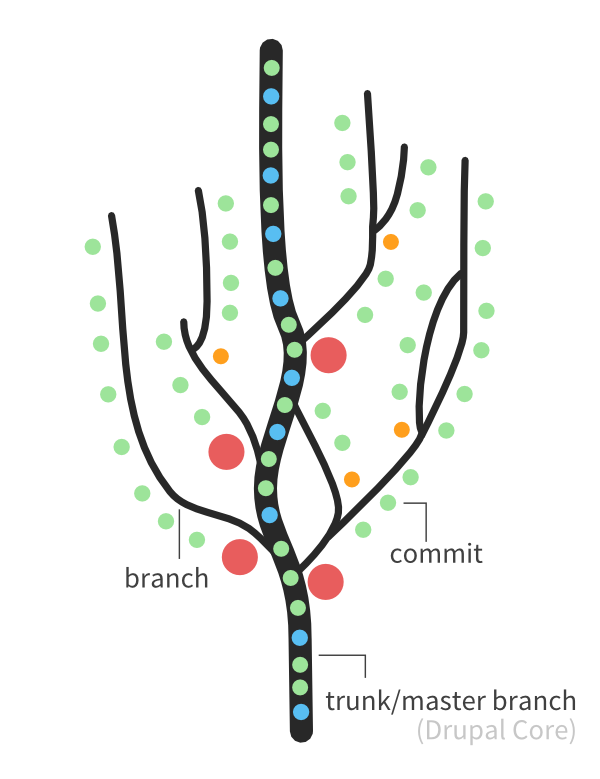
\includegraphics[scale=.5]{./hack1.0-files/repositorydiagram}
\caption{Trunk, branches, and merging visualization of the Drupal project}
\end{figure}

There are several widely used revision control systems including 
CVS (Concurrent Versions System), SVN (Apache Subversion), and 
Git.  SVN is a \emph{centralized} system: there is a single server that 
acts as the main code repository.  Individual developers can check out 
copies and branch copies (which are also stored in the main repository).  

Git is a \emph{distributed} VCS meaning that multiple servers/computers 
act as full repositories.  Each copy on each developer's machine 
\emph{also} contains a complete revision history.  This makes git a 
decentralized system.  Code commits are committed to a local repository.  
Merging a branch into another requires a push/pull request.  
Decentralizing the system means that anyone's 
machine can act as a code repository and can lead to wider collaboration 
and independence since different parties are no longer dependent on 
one master repository.

Git has become the de facto VCS system in software development.  We have
provided several external resources below, but this Hack will walk you
through the basics of getting started.  You will setup a project with 
git using GitHub (\url{https://github.com}) as your remote server.  You
will then collaborate with someone else to commit changes.

\section{Installation}

Support for Git comes standard with Eclipse.  Instead of using
a command line interface, however, you use Eclipse's graphical 
user interface to perform the standard git operations.

\section{Setting Up a Repository}

To focus on the git process, you will create and work with a simple
``Hello World''-style program but instead of printing ``Hello World'', 
it will print your name. 

\begin{enumerate}
  \item Create a new Java project (call it \mintinline{text}{HelloGit}) 
  in Eclipse.  Add a \mintinline{text}{Hello.java} source file with 
  code in it that prints your name.
  
  \item First we need a Git \emph{perspective} (a context in the Eclipse 
  User Interface that will allow us to work with Git). To open the Git 
  perspective, click on the ``Open Perspective'' tab in the upper right:
  	\begin{center}
	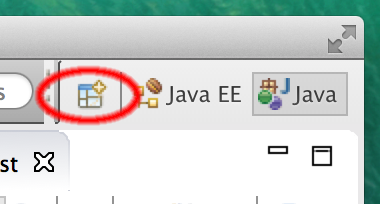
\includegraphics[scale=0.75]{./hack1.0-files/eclipseOpenPerspectiveMarkUp}
	\end{center}
  \item Select ``Git'' from the menu and click OK
  	\begin{center}
	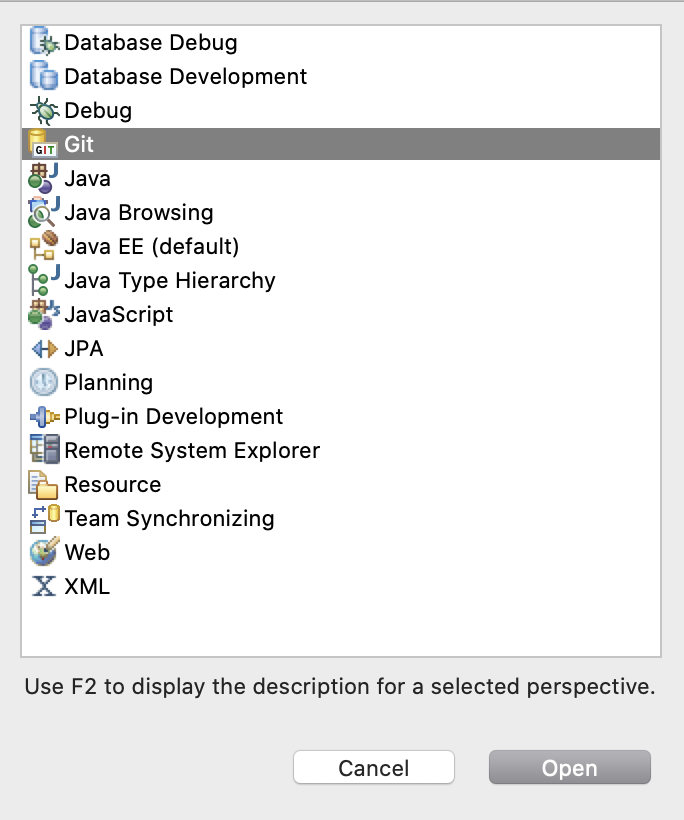
\includegraphics[scale=0.5]{./hack1.0-files/eclipsePerspectiveDialog.png}
	\end{center}
  \item Click the ``Create a new repository and add it to this view'' icon:
  	\begin{center}
	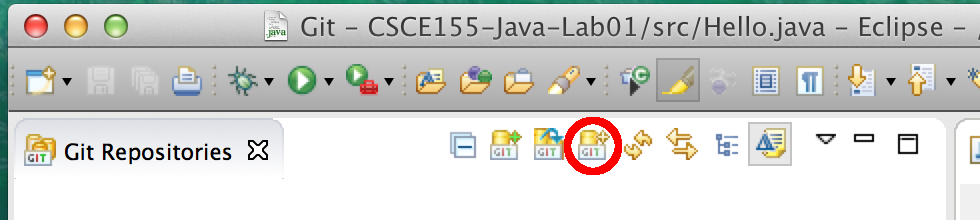
\includegraphics[scale=0.75]{./hack1.0-files/eclipseGitRepoCreateNewMarkUp}
	\end{center}
  \item Select the project folder for the Eclipse project you want to add as a git repo
    	\begin{center}
	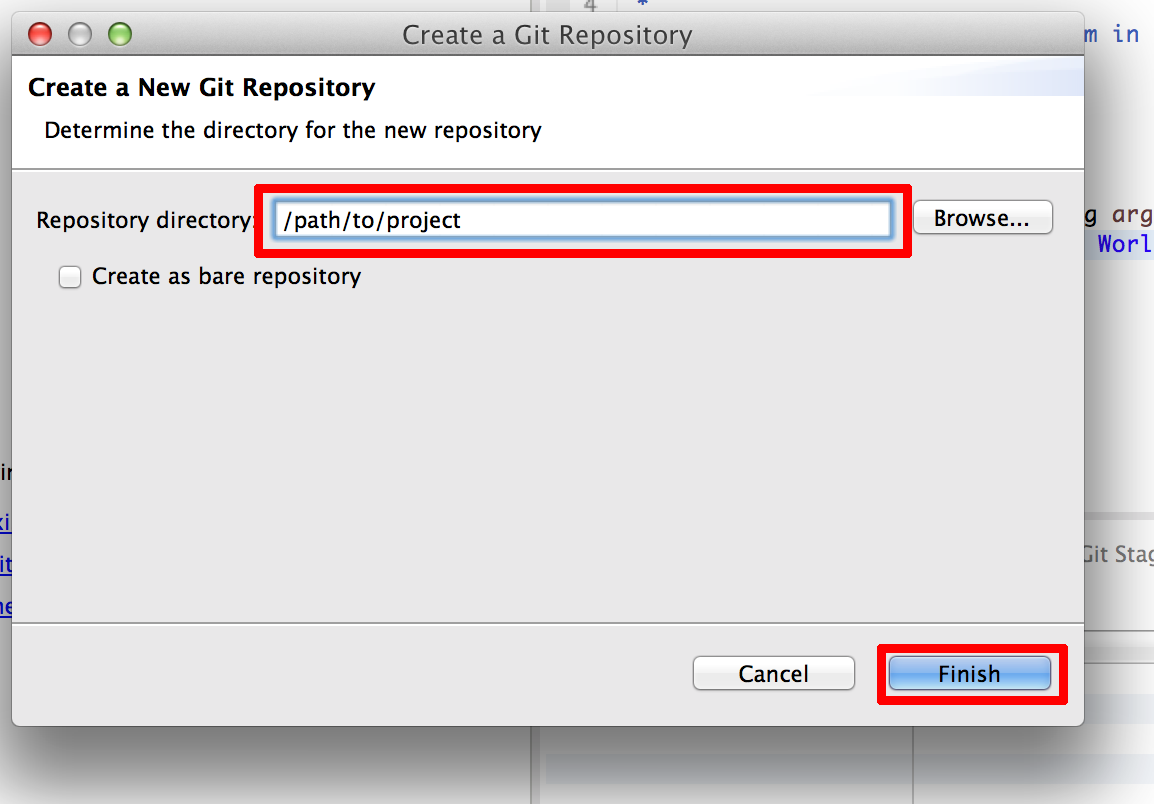
\includegraphics[scale=0.45]{./hack1.0-files/eclipseCreateRepoDialogAMarkUp}
	\end{center}
\end{enumerate}	

\subsection{Git Ignore}

Before we make our first commit, let's setup a \mintinline{text}{.gitignore} 
file.  Often times there will be files or \emph{artifacts} that you want 
to create, save and work with in your project \emph{but} you 
don't want them committed to the repository.  For example, when
you compile your programs you don't want the compiled \mintinline{text}{.class}
files committed to the repository.  The binary files are not part of 
your source code, but an \emph{artifact} of your code.  In general, 
we want git to \emph{ignore} these artifacts.

Eclipse creates a default \mintinline{text}{.gitignore} file when you
create a new repository.  Unfortunately it is not very complete (usually
it only ignores the \mintinline{text}{bin} or ``binary'' directory). 
The following URL has a more comprehensive standard \mintinline{text}{.gitignore}
file for Java Eclipse projects:

\url{https://github.com/github/gitignore/blob/master/Global/Eclipse.gitignore}

Open the \mintinline{text}{.gitignore} file in the ``Git Staging'' tab (see
Figure \ref{fig:gitStaging}, item marked A.) and in the left-hand editor copy-paste
the contents of the \mintinline{text}{.gitignore} file and save.

\subsection{Staging \& Committing} 

Let's continue and make our first commit to our new repository.

\begin{figure}[h]
\centering
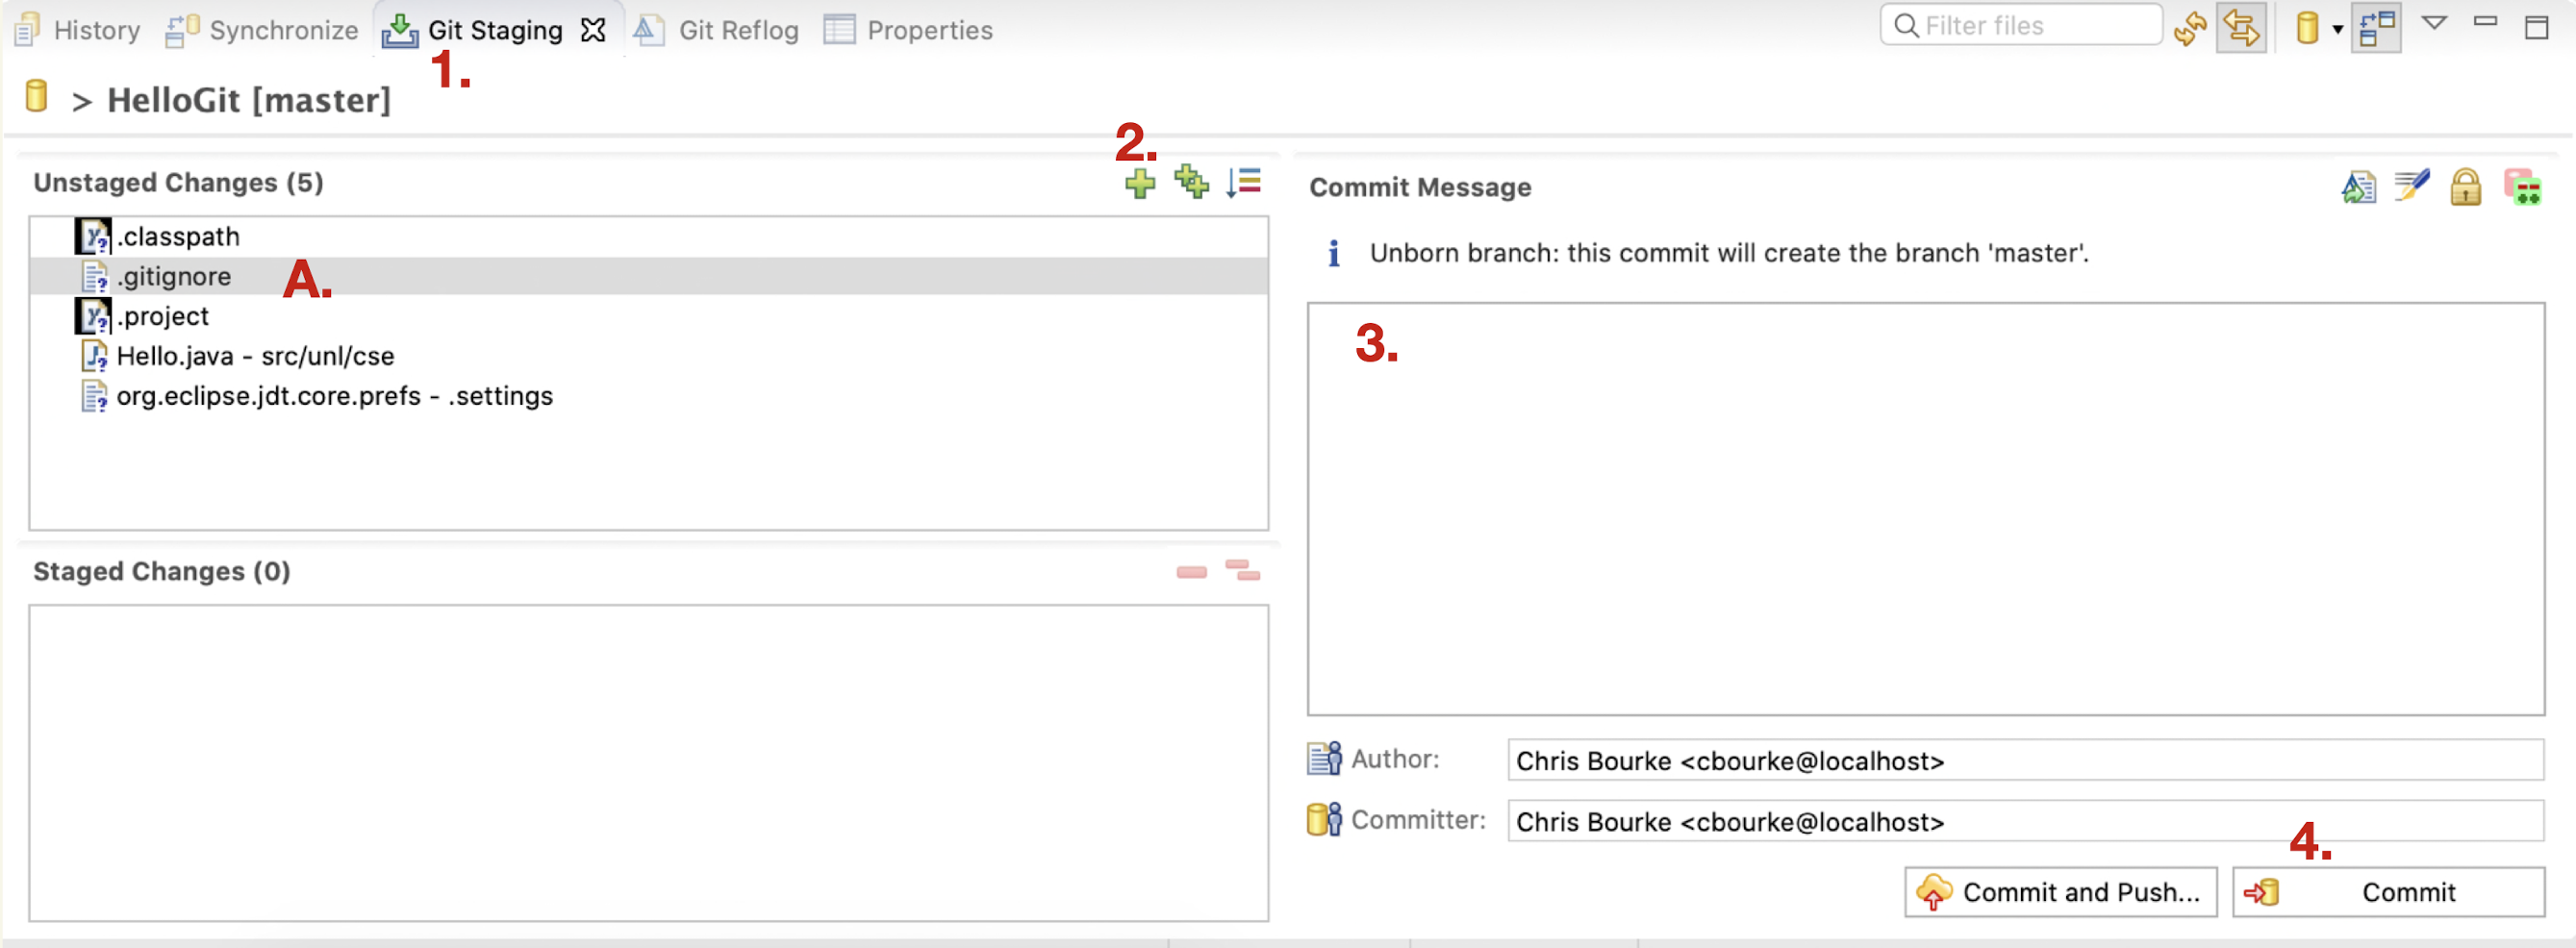
\includegraphics[scale=0.35]{./hack1.0-files/eclipseGitStagingMarkUp}
\caption{Git Staging Tab}
\label{fig:gitStaging}
\end{figure}

\begin{enumerate}  
  \item First, we need to ``stage'' files for our commit.  In the Git Staging
  tab (see Figure \ref{fig:gitStaging}, label 1.), select the file(s) you wish to commit
  and press the plus icon (see label 2.) \emph{or} click the double plus to 
  automatically stage all files at once.  
  
  Note: in general, commits should be as small as possible.  If you make 
  a series of unrelated changes you should make separate commits instead of 
  staging and committing all changes at once.
  
  \item Write a commit message (see label 3.) describing the changes.  For
  this first commit, a commit message of \mintinline{text}{Initial Commit} is good
  enough.  Make future commit message descriptive and thoroughly 
  document the changes that have been made.  
  
  \item Commit the changes by clicking ``Commit'' (see label 4.)
\end{enumerate}

Just prior to committing, your Git Staging tab might look something like:

\begin{center}
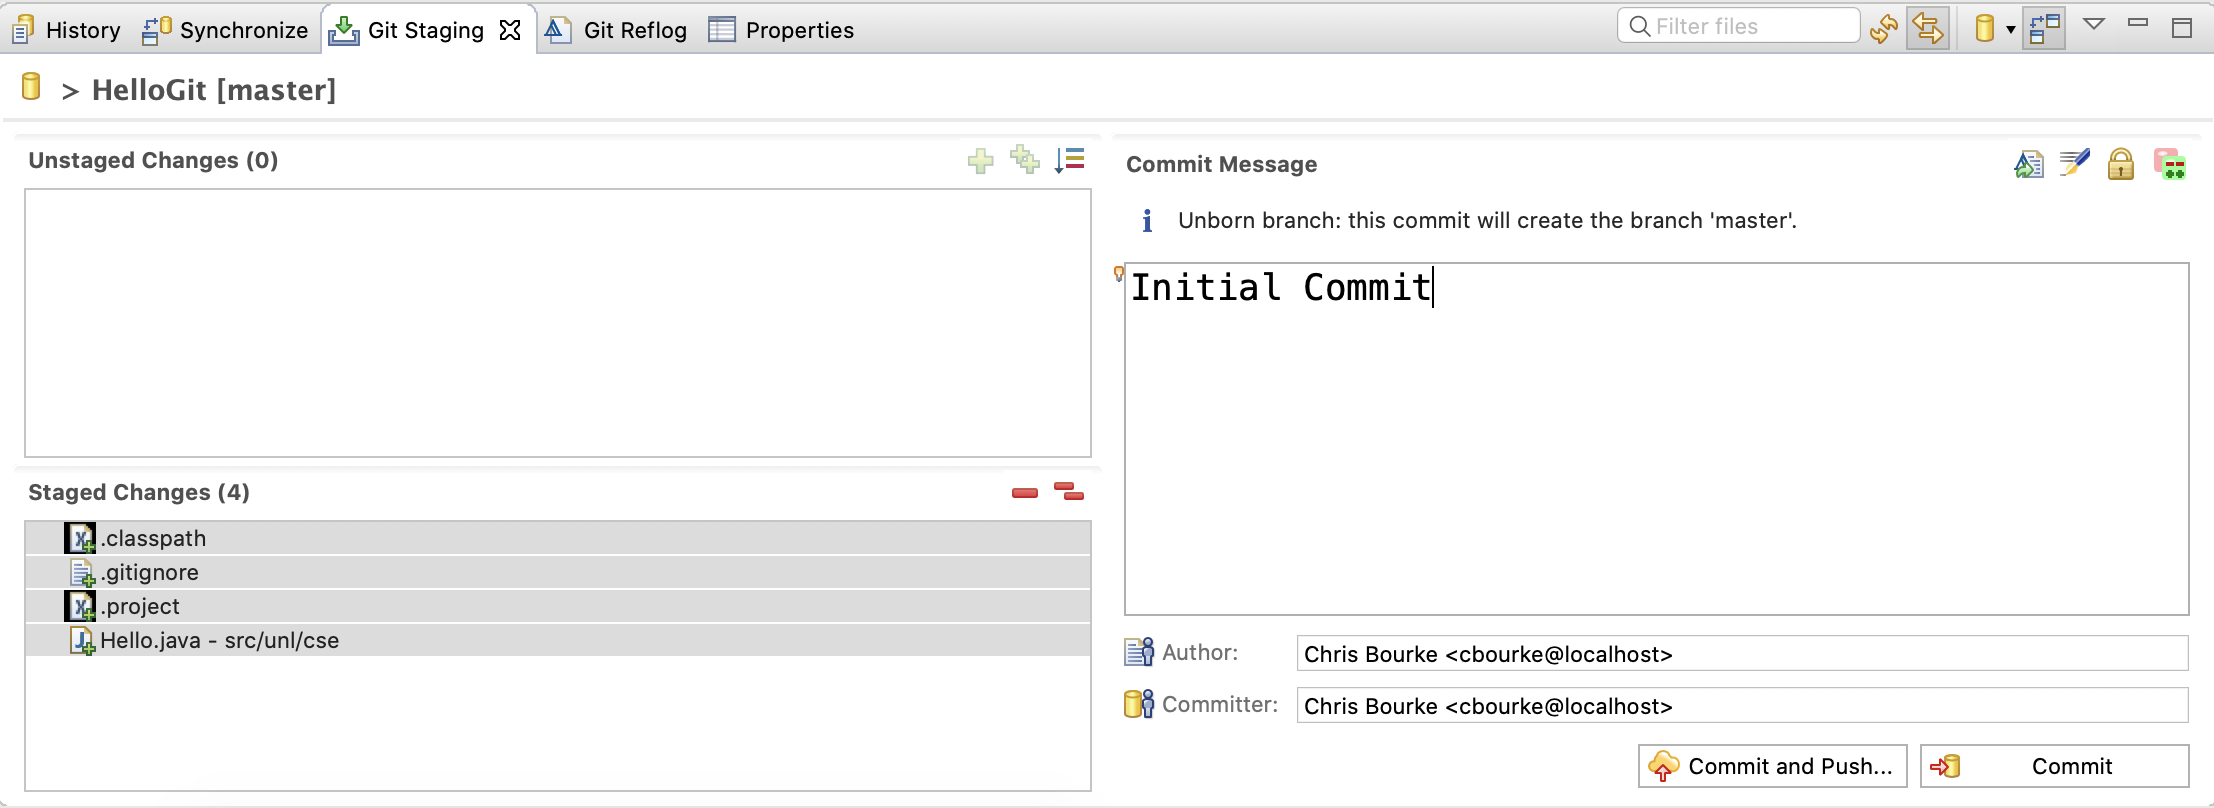
\includegraphics[scale=0.35]{./hack1.0-files/eclipsePreCommit}
\end{center}

\subsection{Pushing Changes}

Though we have committed changes to our repository, those changes are only
to your \emph{local} repository on your own computer.  The changes  
still need to be \emph{pushed} to GitHub.

\subsubsection{Create a Repository on Github}

\begin{enumerate}
  \item Go to your GitHub page (\url{https://github.com/login}
  where \mintinline{text}{login} is replaced with your GitHub
  login) and in the upper right, select \mintinline{text}{New repository}.

  \begin{center}
  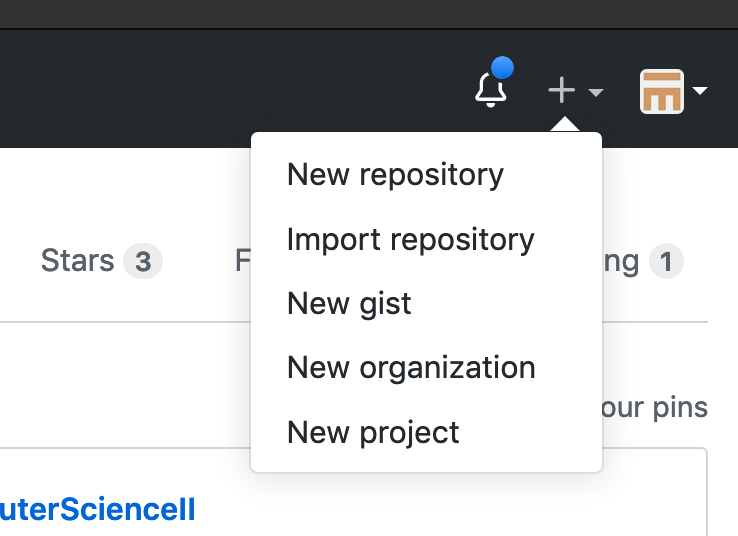
\includegraphics[scale=0.50]{./hack1.0-files/cl-githubNewRepo.png}
  \end{center}

  \item Name your repo \mintinline{text}{HelloGit}
  \begin{center}
  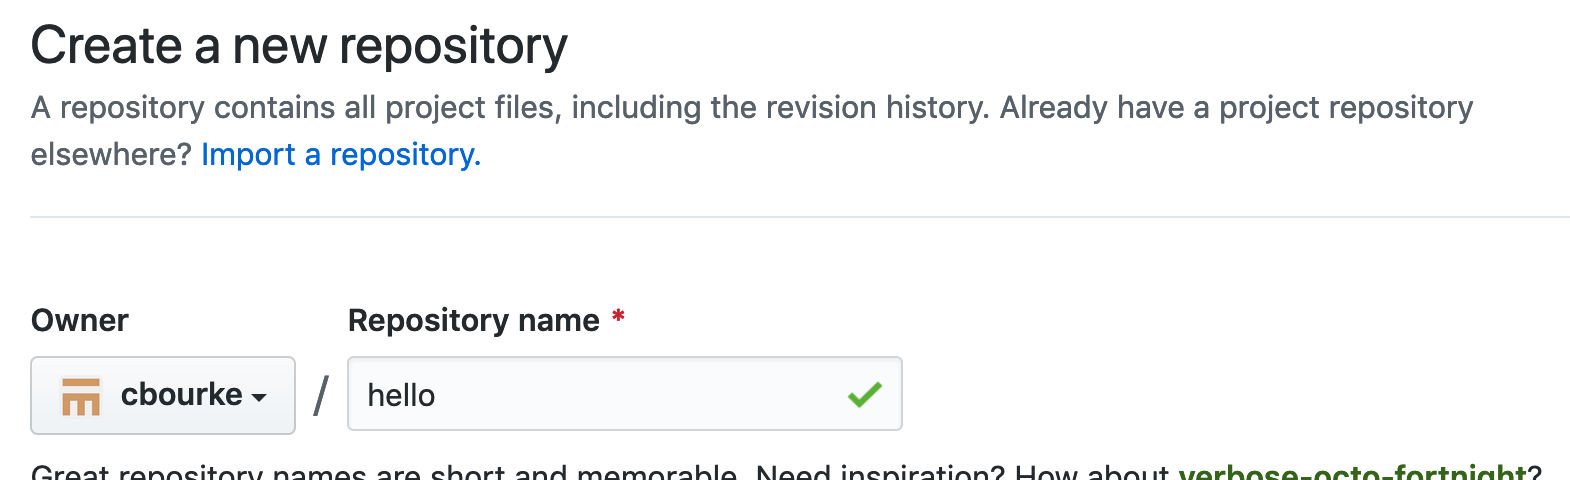
\includegraphics[scale=0.50]{./hack1.0-files/cl-githubNewRepoName.png}
  \end{center}
\end{enumerate}

\subsubsection{Push to Github}

\begin{enumerate}
  \item In Eclipse, go back to your git perspective
  \item Right-click your Git Repository and select ``Push Branch master...''
   \begin{center}
	 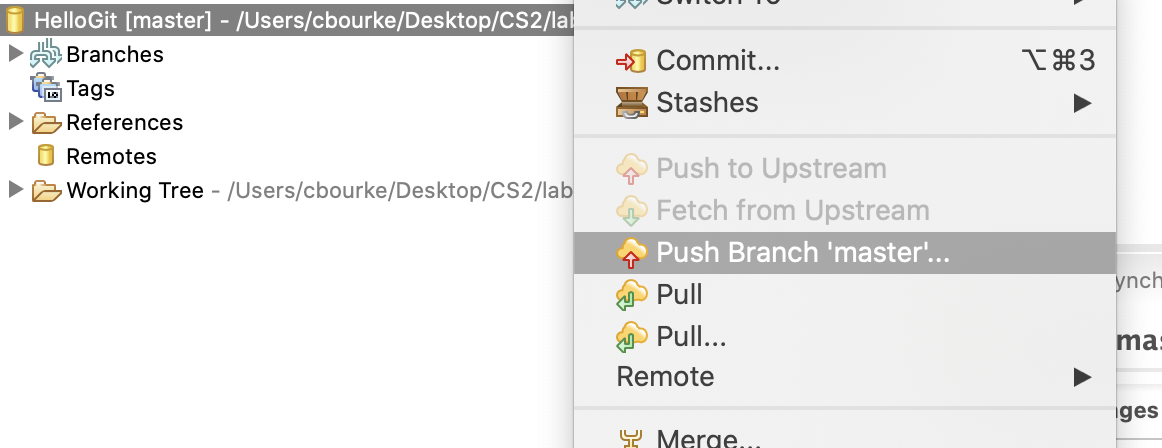
\includegraphics[scale=0.45]{./hack1.0-files/eclipsePush}
   \end{center}
  \item In the dialog, fill out the URI of the repository that you created
  on Github and your \emph{Github} user name and password.
   \begin{center}
	 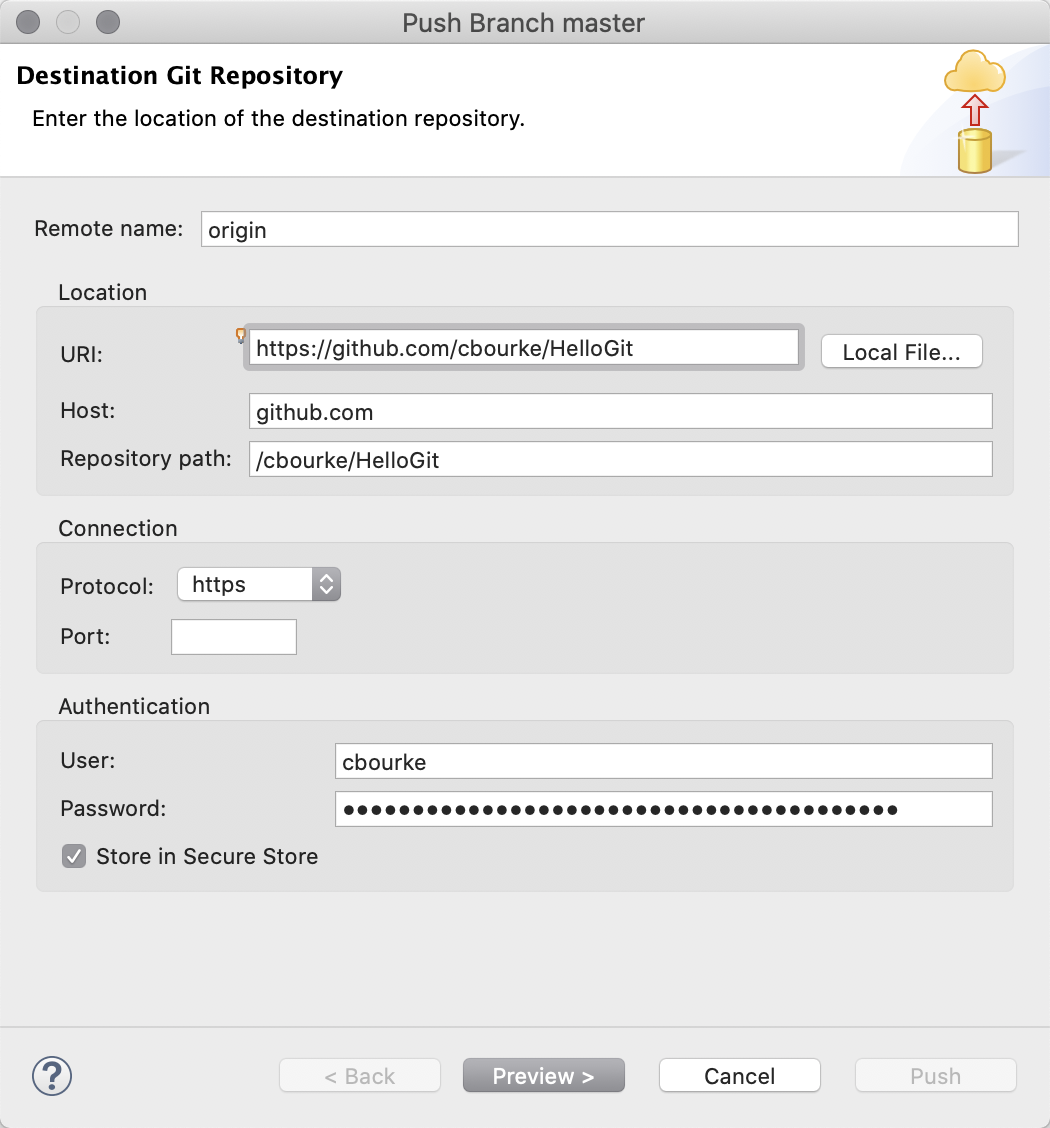
\includegraphics[scale=0.45]{./hack1.0-files/eclipsePushDialog}
   \end{center}
  \item Click preview until you can click ``Push'' to finish.
\end{enumerate}
  
\subsubsection{Making Changes}

\begin{enumerate}
  \item In Eclipse, return to your Java perspective and add a line to your code 
  to print your major.  
  \item Go back to your git perspective and you'll see that the change is 
  reflected in your Git Staging tab.  
  \item Repeat the Commit-Push process to push this change to your Github repo.

  \textbf{NOTE}: you can view the differences in a file before committing them
  by double-clicking on the file!
\end{enumerate}

\section{Collaborating With a Team}

In this exercise, you'll need to team up with at least one other person.
You'll make them a collaborator on your project so they can make changes
and commit/push them to \emph{your} repository on GitHub.  Alternatively
you can have them make a \emph{pull request}, but these instructions do 
not cover that; refer to one of the resources in the 
\hyperref[section:additionalResources]{Additional Resources} section
for how how to make push/pull requests.

\begin{enumerate}
  \item On the GitHub webpage, click \mintinline{text}{Settings} in your project.
  \item In the left menu, click \mintinline{text}{Manage access}
  \item Click \mintinline{text}{Invite a collaborator} and type 
  in your partner's GitHub user name and click \mintinline{text}{Add}
\end{enumerate}

\subsection{What your collaborator needs to do}

Together with your partner, walk through the following steps.  These
steps should be done on \emph{their} computer.

\begin{enumerate}

  \item Once you've sent an invite to collaborate, they need to 
  accept it.
  
  \item Your partner will \emph{clone} your repository in Eclipse

  \item Click the ``Clone a Git repository'' in the Git Repositories navigation menu:
  	\begin{center}
	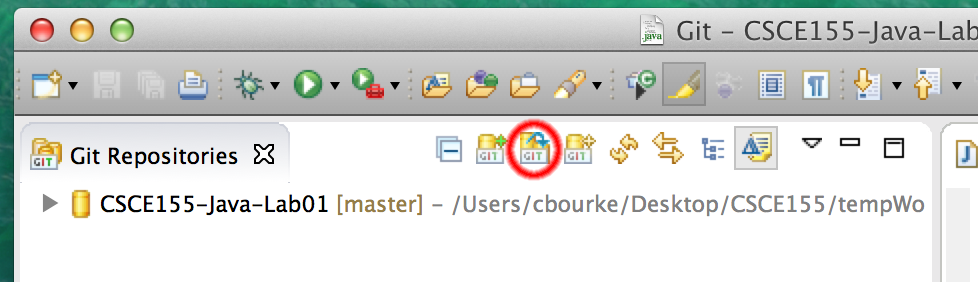
\includegraphics[scale=0.50]{./hack1.0-files/eclipseGitRepoMarkUp}
	\end{center}
  \item Copy/paste or type into the URI field, the URL of the project that 
  	you want to clone, then click ``Next''
	\begin{center}
	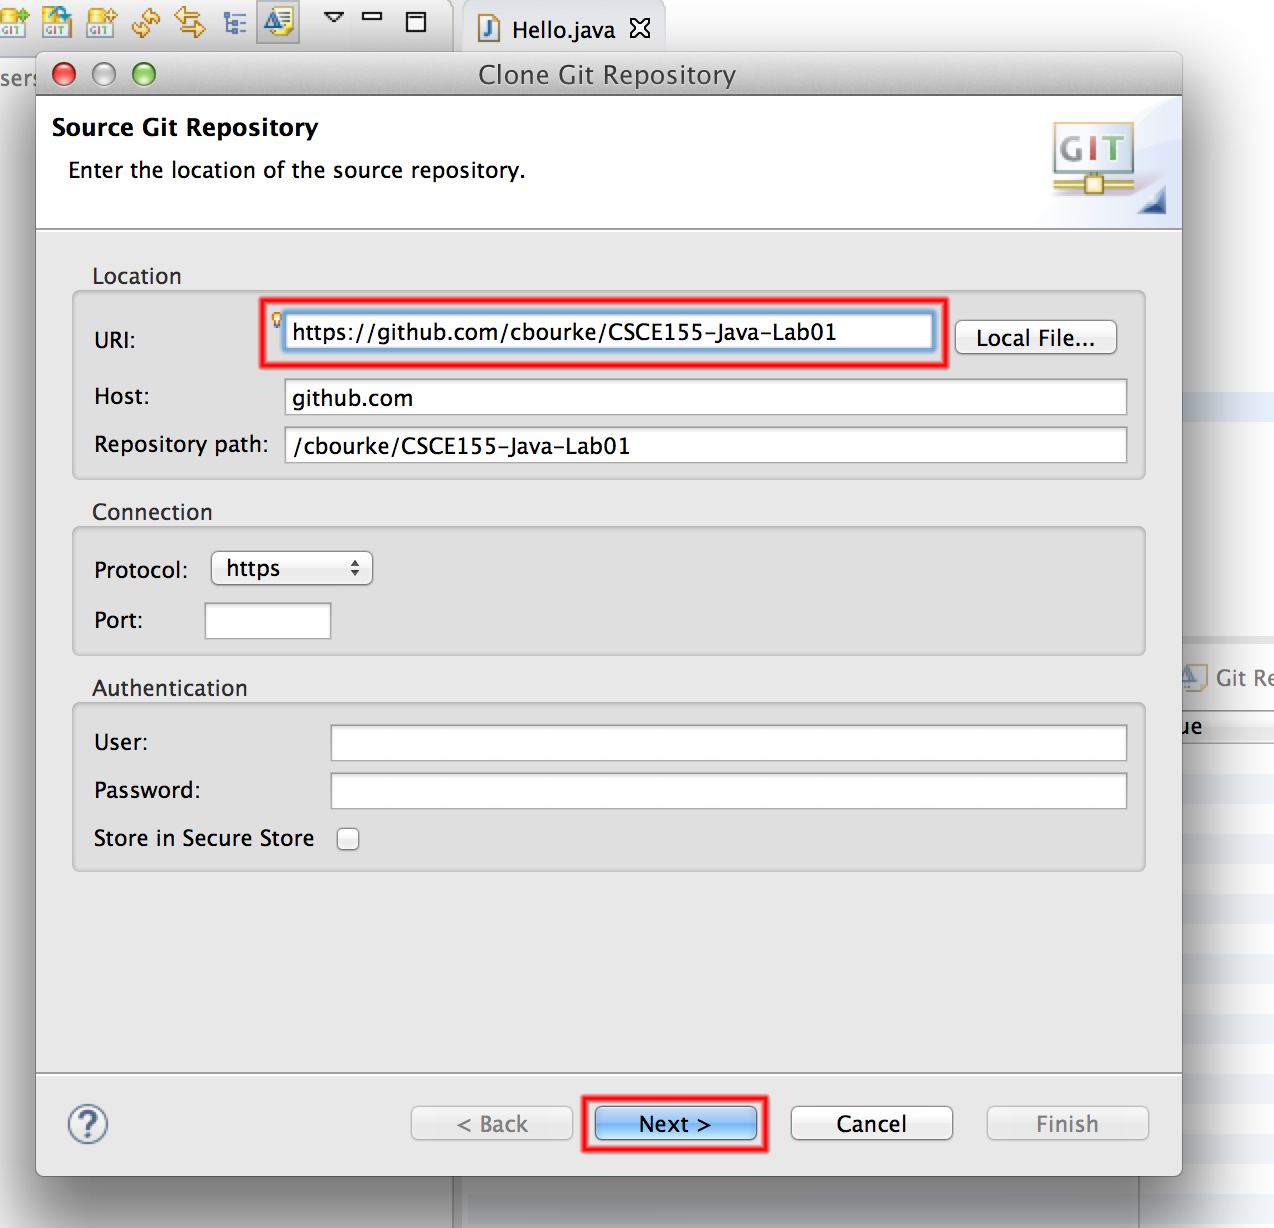
\includegraphics[scale=0.35]{./hack1.0-files/eclipseCloneDialogAMarkUp}
	\end{center}
  \item Once Eclipse has cloned the project, the ``master'' branch should
  	be selected (checkbox); click ``Next'' again.
  	\begin{center}
	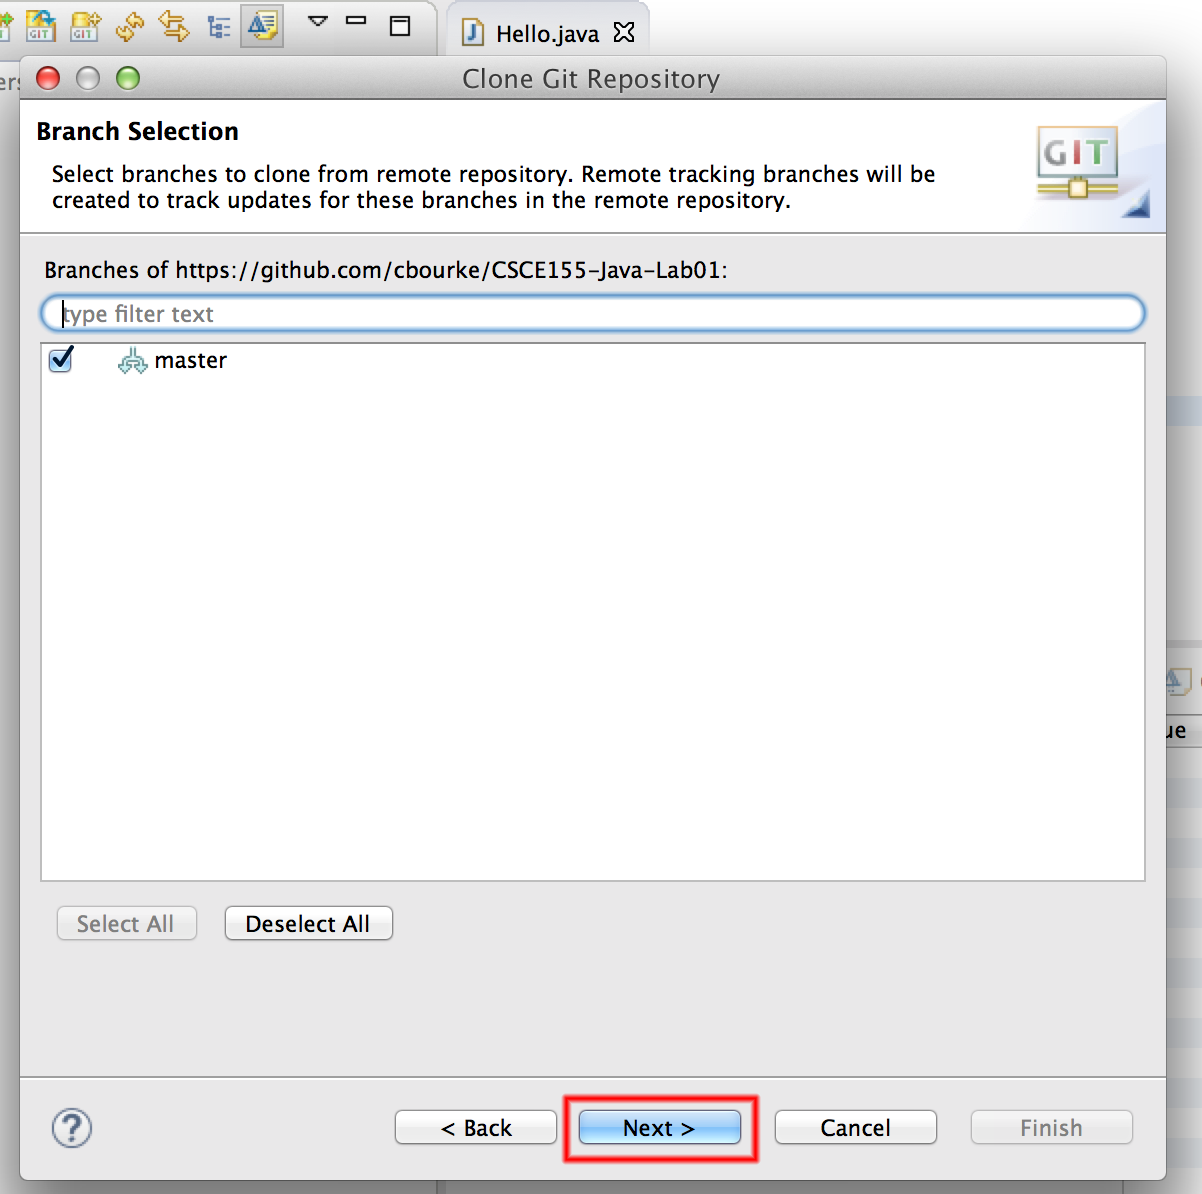
\includegraphics[scale=0.35]{./hack1.0-files/eclipseCloneDialogBMarkUp}
	\end{center}
  \item Select the directory where you want your project to be saved.  Caution: the default
  	option may not correspond to your default workspace.  You will want to change
	it to your workspace.  Also mark the ``Import all existing 
	projects after clone finishes'' checkbox option or you will need
  	to manually import the cloned project into Eclipse.
  	\begin{center}
	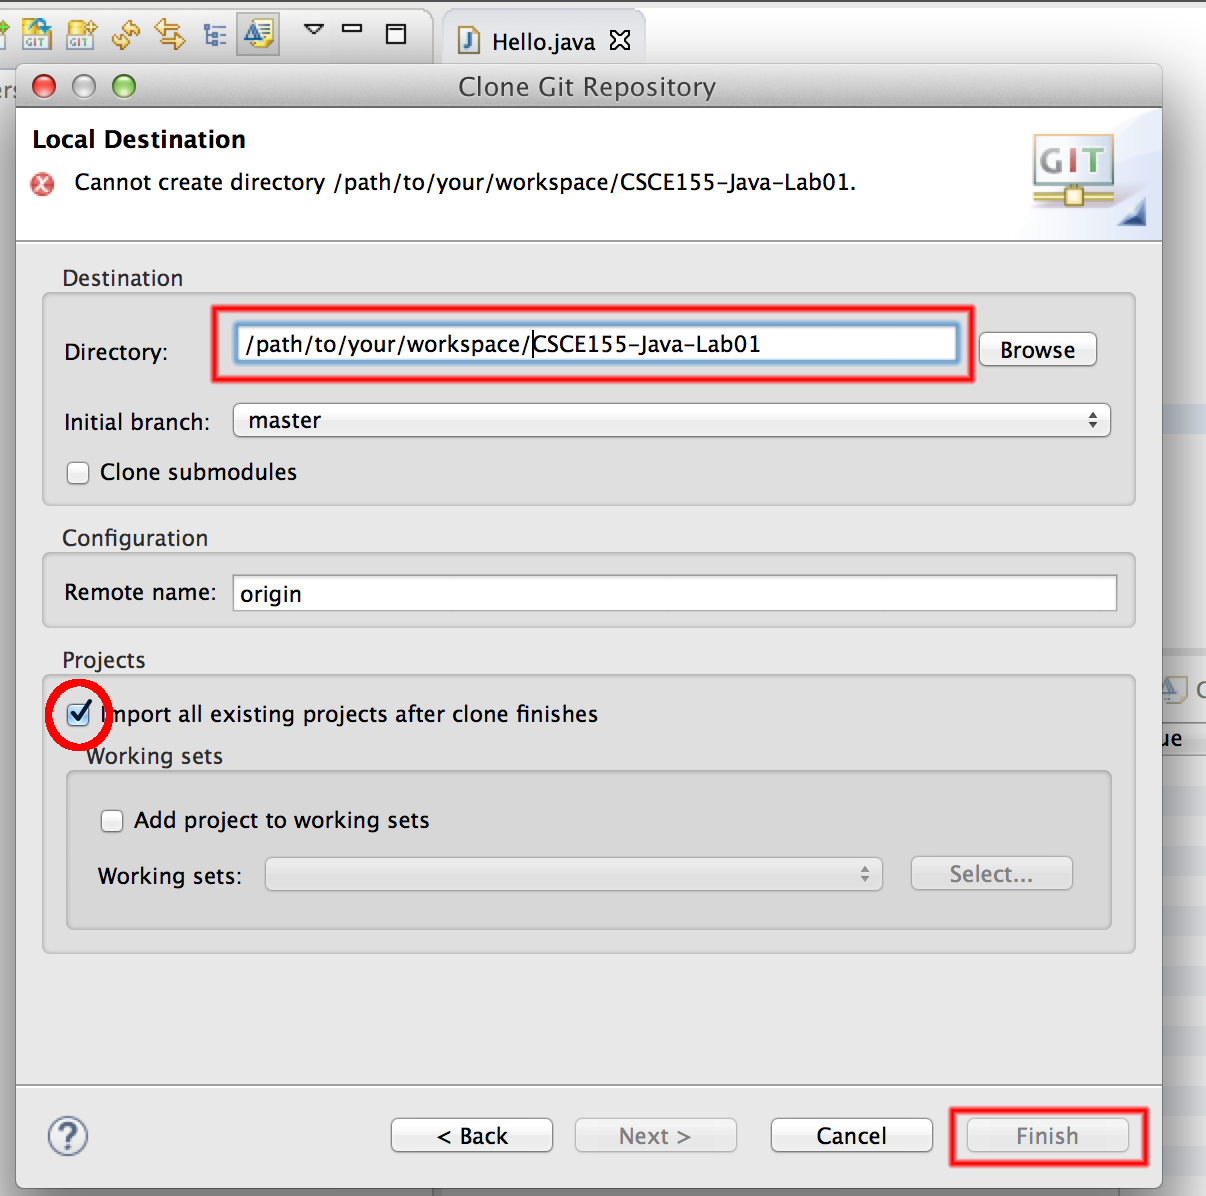
\includegraphics[scale=0.35]{./hack1.0-files/eclipseCloneDialogCMarkUp}
	\end{center}
  \item Switch back to your Java perspective and you can see your cloned 
  	project.  
  \item Your partner should add 2 lines of code to 
  print their name and their major.
  
  \item Your partner should follow the same procedure to commit 
  and push their changes to \emph{your remote} repository using 
  the same procedure as they did with theirs.
  
  \item Verify their changes by refreshing your repository on
  GitHub.  If you did everything correctly you should be able 
  to see the changes in the file as well as multiple commits by
  multiple individuals.  If you click on \mintinline{text}{History} 
  you can see the changes for each commit.

\end{enumerate}

\subsection{Pull Changes}

Now, go back to \emph{your} Eclipse.  Remember, your partner's
changes were \emph{pushed} to your \emph{remote} repository hosted
on GitHub.  If you look at the code on your own computer you 
won't see their changes because this is your \emph{local}
repository.  

In order to get your partner's changes you'll need to \emph{pull}
their changes from your remote repository to your local repository.
To do this: 

\begin{enumerate}
  \item Change to your git perspective
  \item Right click your repository and select ``Pull''
  	\begin{center}
	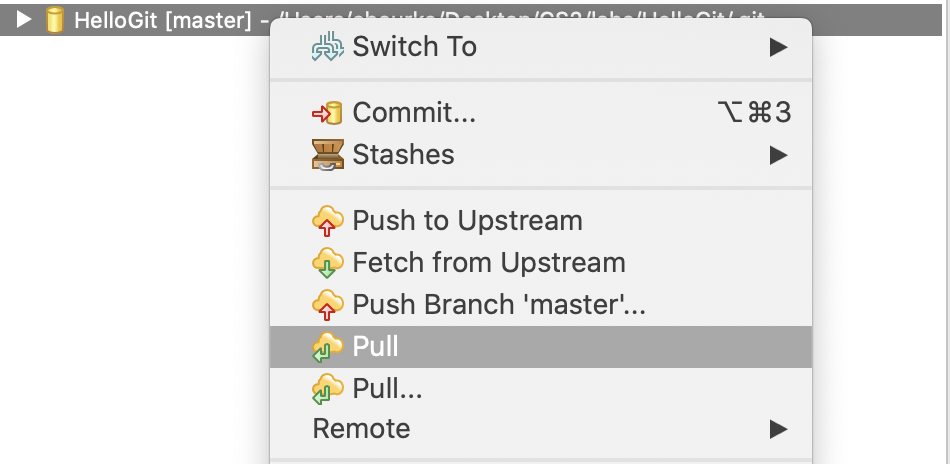
\includegraphics[scale=0.35]{./hack1.0-files/eclipseGitPull}
	\end{center}
  \item If successful a dialog will popup that looks something like this.
  	\begin{center}
	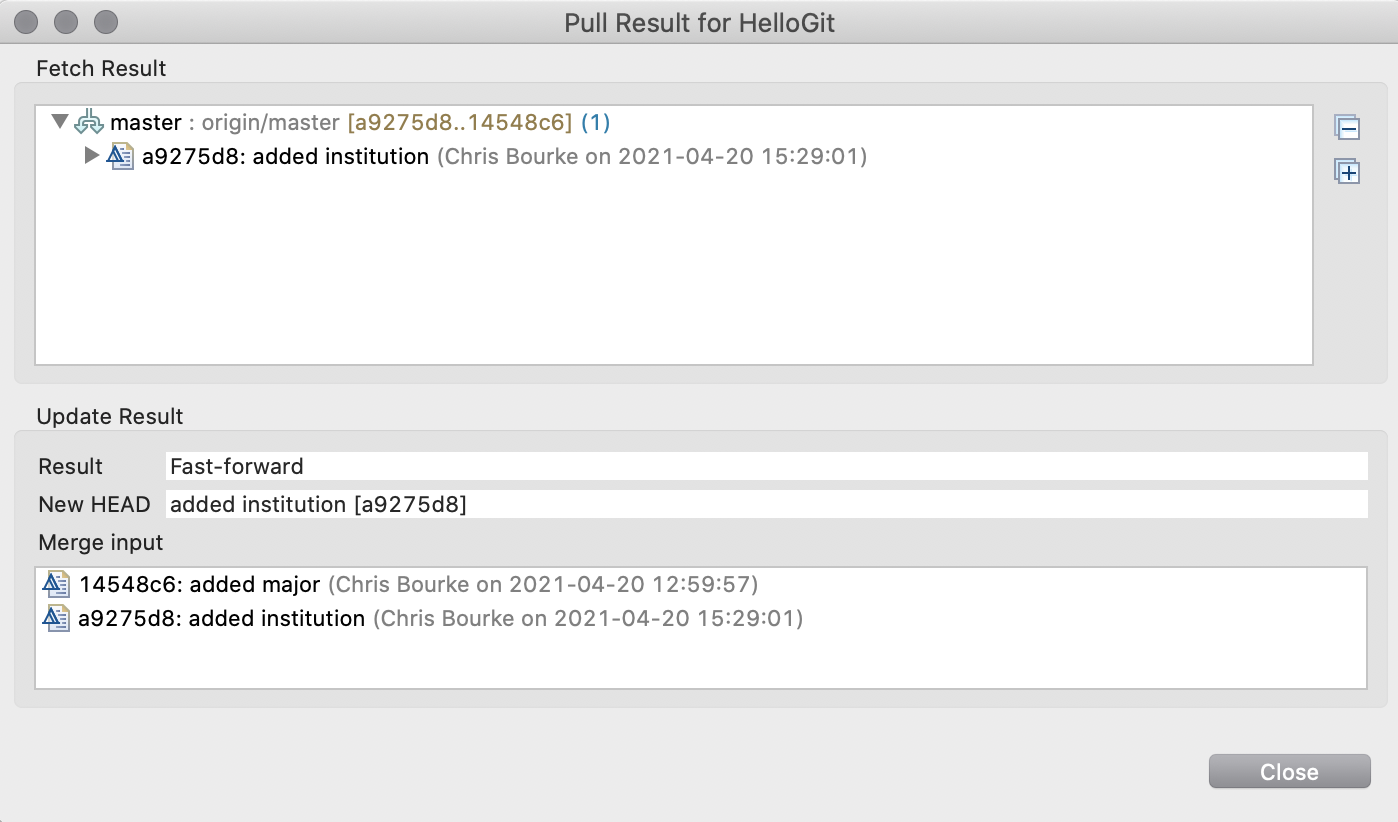
\includegraphics[scale=0.35]{./hack1.0-files/eclipseGitPullResult}
	\end{center}
  \item Change back to your Java perspective and you can observe the
  changes.

\end{enumerate}

\subsection{Finishing Up}

\begin{enumerate}
  \item Put \emph{your} GitHub URL into a plain text file named 
  \mintinline{text}{readme.md}.  Turn this file
  in using webhandin.  Each individual student will need
  to hand in their own copy and will receive their own individual
  grade.
  \item Verify what you handed in by running the webgrader which will
  display the contents of your file.
\end{enumerate}

\section*{Additional Instructions}

\begin{itemize}
  \item You are encouraged to collaborate with any number of students 
  before, during, and after your scheduled hack session.    
  \item Each student is responsible for \emph{their} repository, so 
  when you team up with a partner, you'll need to go through this
  Hack at least twice: once as the primary repository owner and once as
  a collaborator.
\end{itemize}
  
\section*{Additional Resources}
\label{section:additionalResources}

\begin{itemize} 
  \item My video tutorial for using Eclipse/git (from CS2): \url{https://www.youtube.com/watch?v=8bjtf6TZZGA&list=PL4IH6CVPpTZXOMCZRaFy_WRc-GvANOZfk&index=2}
  \item Interactive git tutorial: \url{https://try.github.io/levels/1/challenges/1}
  \item Pro Git, free online book: \url{https://git-scm.com/book/en/v2}
\end{itemize}


  


\end{document}
